% % \DocumentMetadata{testphase={phase-III,math,table}}
\documentclass[12pt]{article}
\input{preamble}
\input{config}


\begin{document}
\begin{center}
    \color{BlueViolet}

     \textbf{\newline\newline}
    \vspace{6pt}
    \large
    \textbf{\\HO CHI MINH UNIVERSITY OF SCIENCE}
    

    
    \vspace{6pt}
    \large
    \textbf{\\FACULTY OF INFORMATION TECNOLOGY}

    \vspace{6pt}
    \large
    \textbf{\\DATA SECURITY IN INFORMATION SYSTEMS}
   
\end{center}

\begin{center}
    
\includegraphics[scale=0.25,alt={Logo of HCMUS}]{images/Logo_HCMUS.png}
    \color{BlueViolet}
    
   \large
   \textbf{THEORY REPORT} \\
   \textbf{CHAPTER 8: MALWARE}
    \vspace{25pt}\\

    \color{BlueViolet}
    \textbf{LECTURER:} 
    \color{Black}
    \\ Phạm Thị Bạch Huệ - Lương Vĩ Minh
    \vspace{15pt}\\


    \color{BlueViolet}
    \textbf{STUDENT (GROUP 7):}
    \color{Black}
    \\ {Đởm Quang Minh Triết - 23127131}
    \\ {Đinh Đại Vũ - 23127144}
    \\ {Lê Phạm Kiều Duyên - 23127184}
    \\ {Lê Trương Bảo Ngọc - 23127237}
    \\ {Nguyễn Đăng Phôn - 23127451}	
    \vspace{25pt}\\

\end{center}

\begin{tikzpicture}[remember picture,overlay,inner sep=0,outer sep=0]
     \draw[blue!70!black,line width=4pt] ([xshift=-1.5cm,yshift=-2cm]current page.north east) coordinate (A)--([xshift=1.5cm,yshift=-2cm]current page.north west) coordinate(B)--([xshift=1.5cm,yshift=2cm]current page.south west) coordinate (C)--([xshift=-1.5cm,yshift=2cm]current page.south east) coordinate(D)--cycle;

     \draw ([yshift=0.5cm,xshift=-0.5cm]A)-- ([yshift=0.5cm,xshift=0.5cm]B)--
     ([yshift=-0.5cm,xshift=0.5cm]B) --([yshift=-0.5cm,xshift=-0.5cm]B)--([yshift=0.5cm,xshift=-0.5cm]C)--([yshift=0.5cm,xshift=0.5cm]C)--([yshift=-0.5cm,xshift=0.5cm]C)-- ([yshift=-0.5cm,xshift=-0.5cm]D)--([yshift=0.5cm,xshift=-0.5cm]D)--([yshift=0.5cm,xshift=0.5cm]D)--([yshift=-0.5cm,xshift=0.5cm]A)--([yshift=-0.5cm,xshift=-0.5cm]A)--([yshift=0.5cm,xshift=-0.5cm]A);


     \draw ([yshift=-0.3cm,xshift=0.3cm]A)-- ([yshift=-0.3cm,xshift=-0.3cm]B)--
     ([yshift=0.3cm,xshift=-0.3cm]B) --([yshift=0.3cm,xshift=0.3cm]B)--([yshift=-0.3cm,xshift=0.3cm]C)--([yshift=-0.3cm,xshift=-0.3cm]C)--([yshift=0.3cm,xshift=-0.3cm]C)-- ([yshift=0.3cm,xshift=0.3cm]D)--([yshift=-0.3cm,xshift=0.3cm]D)--([yshift=-0.3cm,xshift=-0.3cm]D)--([yshift=0.3cm,xshift=-0.3cm]A)--([yshift=0.3cm,xshift=0.3cm]A)--([yshift=-0.3cm,xshift=0.3cm]A);

\end{tikzpicture}
\newpage
\renewcommand{\contentsname}{\textbf{Contents}}

\tableofcontents

\newpage
\listoffigures
\listoftables

\newpage
\newpage
\section*{Group Members}

\begin{table}[H]
\centering
\renewcommand{\arraystretch}{1.5}
    \begin{tabularx}{\textwidth}{|c|X|c|X|}
    \hline
    \textbf{No.} & \textbf{Full Name} & \textbf{Student ID} & \textbf{Email} \\ \hline
    1 & Đởm Quang Minh Triết & 23127131 & dqmtriet23@clc.fitus.edu.vn \\ \hline
    2 & Đinh Đại Vũ & 23127144 & ddvu23@clc.fitus.edu.vn \\ \hline
    3 & Lê Phạm Kiều Duyên & 23127184 & lpkduyen23@clc.fitus.edu.vn \\ \hline
    4 & Lê Trương Bảo Ngọc & 23127237 & ltbngoc23@clc.fitus.edu.vn \\ \hline
    5 & Nguyễn Đăng Phôn & 23127451 & ndphon23@clc.fitus.edu.vn \\ \hline
    \end{tabularx}
\caption{List of group members}
\label{tab:thongtin}
\end{table}

\vspace{1cm}
\renewcommand{\arraystretch}{1.5}
\section*{Task Distribution and Completion Status}

\begin{table}[H]
    \centering
    \resizebox{\textwidth}{!}{
        \begin{tabular}{|c|l|l|c|c|}
        \hline
        \textbf{No.} & \textbf{Task} & \textbf{Responsible} & \textbf{Student ID} & \textbf{Contribution} \\ \hline
        1 & Defense and Mitigation Strategies &
        Đởm Quang Minh Triết & 23127131 & 20\% \\ \hline

        2 &  &
        Đinh Đại Vũ & 23127144 & 20\% \\ \hline

        3 &  &
        Lê Phạm Kiều Duyên & 23127184 & 20\% \\ \hline

        4 &  &
        Lê Trương Bảo Ngọc & 23127237 & 20\% \\ \hline

        5 &  &
        Nguyễn Đăng Phôn & 23127451 & 20\% \\ \hline
        \end{tabular}
    }
    \caption{Task distribution and completion status}
    \label{tab:phancong}
\end{table}





\newpage
\section{Introduction and Scope of Research}

\newpage
\section{Classification and Architecture of Malicious Software}

\newpage
\section{Vulnerabilities and Malware Enablers}

To better understand how malware operates, it is crucial to examine the methods and techniques used by attackers. These techniques exploit system vulnerabilities, allowing malicious code to infiltrate systems and cause harm. In this section, we explore common attack methods and analyze how malware targets computer systems and networks.

\subsection{Active Content Vulnerabilities}

\paragraph{Definition.}
Active content refers to components, primarily on web pages, that provide functionality for interacting with users. This includes any dynamic object that performs an action when a user opens a web page. Common technologies used to implement active content include ActiveX, Java, JavaScript, VBScript, scripts, browser plug-ins, and PDF files.

\paragraph{How It Works.}
Active content is considered a form of mobile code because it can execute across different computing platforms. When a user visits a website, the web browser downloads this code and executes it within the browser's context, using the user's credentials and privileges. Once downloaded, the mobile code may gain access to local system resources, including the computer's hard drive.

\paragraph{Attack Techniques.}
Attackers exploit weaknesses in active content mechanisms to execute malicious code. A common attack technique is Cross-Site Scripting (XSS), which allows attackers to inject client-side scripts into web pages viewed by users. When a user accesses such a page, the browser automatically executes the malicious script, often bypassing access control mechanisms.

\paragraph{Impact.}
Malicious active content can cause severe consequences, such as flooding the desktop with icons representing malware-infected files. These files may continue to replicate and generate additional copies of the malicious code. The overall impact depends on the sensitivity of the compromised system and the data it contains.

\paragraph{Prevention.}
\begin{itemize}
  \item Browser configuration: Configure browser security settings to block or warn users before executing scripts or dynamic content.
  \item Content filtering: Implement network-level filtering to analyze traffic, identify dynamic code components (e.g., Java or ActiveX), and disable script processing within web browsers.
  \item Pop-up blocking: Require users to enable pop-up blockers to prevent automatic pop-up windows and reduce the risk of unintentional malware execution.
\end{itemize}

\subsection{Homepage Hijacking}

\paragraph{Definition.}
Homepage hijacking is a type of attack that alters a web browser's homepage configuration so that it redirects users to a website chosen by the attacker.

\paragraph{How It Works.}
This attack resets the browser's homepage settings, typically without the user's permission. Attackers may install hidden programs that preserve the malicious configuration even when the user attempts to restore the original homepage.

\paragraph{Attack Techniques.}
Attackers commonly use the following methods to perform homepage hijacking:

\begin{itemize}
  \item Exploiting browser vulnerabilities: Taking advantage of security flaws in web browsers or active content components to modify homepage settings.
  \item Social engineering: Tricking users into performing actions that appear beneficial but actually initiate malware execution (e.g., fake buttons claiming to remove infections).
  \item Browser Helper Objects (BHOs): Installing Trojan programs in the form of BHOs that register themselves in the system startup process and execute automatically each time the system boots.
\end{itemize}

\paragraph{Impact.}
\begin{itemize}
  \item The browser repeatedly opens the attacker's website instead of the user's preferred homepage.
  \item Persistent annoyance and loss of control, as hijacking programs continuously reset the homepage until the malware is fully removed.
\end{itemize}

\paragraph{Prevention.}
\begin{itemize}
  \item Exercise caution when interacting with websites, especially when clicking buttons or links from unknown or untrusted sources.
  \item Review system startup processes and remove suspicious or unauthorized entries.
  \item Fully identify and eliminate malicious programs or Browser Helper Objects to prevent repeated homepage changes.
\end{itemize}

\subsection{Webpage Defacements}

\paragraph{Definition.}
Webpage defacement (also known as web graffiti) is the act of gaining unauthorized access to a web server and altering the content of the index page or other web pages hosted on that server.

\paragraph{How It Works.}
Attackers typically target publicly accessible web servers on the Internet. The attack process involves identifying and exploiting known security vulnerabilities to gain administrative or elevated access. Once control is obtained, the attackers replace legitimate web pages with modified or malicious versions.

\paragraph{Attack Techniques.}
\begin{itemize}
  \item Exploiting software vulnerabilities: Attackers exploit security flaws in the server's operating system or service applications (e.g., vulnerabilities in web servers) to gain unauthorized access.
  \item Installing backdoors: Some malware installs Trojan backdoors after infection, enabling attackers to remotely access the server and alter website content at any time.
  \item Using automated tools: Script kiddies and organized hacker groups often use automated vulnerability-scanning tools to identify poorly secured websites before launching attacks.
\end{itemize}

\paragraph{Impact.}
\begin{itemize}
  \item Defacement and nuisance: Webpage defacement is often considered a form of digital graffiti that disrupts normal website operations.
  \item Reputational damage: Defaced websites may display offensive messages or inappropriate content, damaging organizational credibility and user trust.
  \item Serious security risks: Attackers may embed malicious active content, such as viruses or Trojan programs, exposing visitors to further compromise.
\end{itemize}

\paragraph{Prevention.}
\begin{itemize}
  \item Software updates: Keep web server operating systems and applications up to date with the latest security patches.
  \item Disabling unnecessary services: Turn off unused services and close unneeded network ports to reduce attack surfaces.
  \item Network defense layers: Use proxy servers or bastion hosts to protect critical services and filter malicious traffic.
  \item Monitoring and testing: Conduct regular vulnerability assessments and penetration testing to identify and remediate weaknesses proactively.
\end{itemize}


\newpage
\section{Attack Vectors}

Attack vectors refer to the methods or pathways used by attackers to gain unauthorised access to systems, networks, or data. Understanding attack vectors is critical for analysing how attacks are initiated and for designing effective defensive strategies. Common attack vectors exploit human behaviour, technical vulnerabilities, or weaknesses in system availability.

\subsection{Social Engineering and Phishing}

Social engineering attacks exploit human psychology rather than technical vulnerabilities to gain access to sensitive information or systems. Attackers manipulate victims into revealing credentials, downloading malicious files, or performing actions that compromise security. Phishing is one of the most prevalent forms of social engineering and typically involves deceptive emails, messages, or websites that impersonate legitimate entities. These attacks often create a sense of urgency or authority to pressure victims into compliance. Due to their reliance on human error, social engineering and phishing attacks remain highly effective despite advancements in technical security controls.

Real-world example: The Twilio Breach (2022). Attackers sent SMS messages to Twilio employees pretending to be the IT department, urging them to update their passwords or review new schedules. The texts contained the employee's actual names and legit-looking URLs leading to a fake Twilio sign-in page. Some workers tried to log in, revealing their user credentials [3].

\subsection{Spam-Based Attacks}

Spam-based attacks involve the mass distribution of unsolicited messages containing malicious links, attachments, or payloads. Unlike targeted phishing campaigns, spam-based attacks are typically indiscriminate and aim to infect a large number of systems with minimal effort. These attacks are commonly used to spread malware, ransomware, or trojans and often rely on at least some recipients interacting with the malicious content. Spam-based attacks are frequently used as an initial delivery mechanism in larger attack campaigns.

Real-world example: The Emotet Botnet. Before its disruption, Emotet was the world's most dangerous malware distributor, largely spreading via massive spam campaigns containing malicious Word documents (fake invoices or shipping receipts). It served as the primary delivery mechanism for other ransomware like Ryuk [4].

\subsection{Software Vulnerability Exploitation}

Software vulnerability exploitation occurs when attackers take advantage of flaws in operating systems, applications, or network services. These vulnerabilities may arise from coding errors, misconfigurations, or outdated software lacking security patches. Attackers often use automated tools or exploit frameworks to identify and exploit known vulnerabilities, although advanced attackers may leverage zero-day vulnerabilities that have not yet been publicly disclosed. Successful exploitation can lead to unauthorized access, privilege escalation, or remote code execution.

Real-world example: Log4Shell (CVE-2021-44228). Discovered in late 2021, this critical vulnerability affected Apache Log4j, a widely used logging library in Java applications. At the peak of Log4Shell activity, Check Point observed more than 100 attacks every minute, affecting more than 40\% of all business networks globally [5] [6].

\subsection{Denial of Service (DoS/DDoS)}

Denial of Service (DoS) and Distributed Denial of Service (DDoS) attacks aim to disrupt the availability of systems or services by overwhelming them with excessive traffic or resource requests. In a DDoS attack, multiple compromised systems, often part of a botnet, are used to amplify the attack's impact. These attacks do not necessarily involve data theft but can cause significant operational and financial damage by rendering services inaccessible to legitimate users.

Real-world example: The Dyn Cyberattack (2016). The Mirai Botnet, composed of insecure IoT devices (cameras, routers), launched a massive DDoS attack against Dyn (a DNS provider). This attack successfully took down major platforms like Twitter, Netflix, and Reddit for hours, highlighting the power of volumetric attacks [7].

[8]


\newpage
\section{Anatomy of an Attack}

In order to develop practical and efficacious countermeasures, it is essential that the objectives, the key targets, and the characteristics of an attack must be known.

\subsection{What Motivates Attackers?}

Contrary to popular belief, today's attackers are not merely socially marginalised individuals driven by thrill-seeking impulses or amateur experimentation. There is much more complexity to the reasons behind attacks, namely:

\begin{itemize}
  \item Monetary gain:
  \begin{itemize}
    \item Objective: To generate illicit profit through theft or extortion.
    \item A real-life example: Hieu Ngo Minh, also known as Hieu PC, a Vietnamese hacker who was formerly involved in identity-theft operations, stole and sold large volumes of personally identifiable information, including millions of U.S. Social Security numbers by exploiting the vulnerabilities of the systems. His activities generated substantial illegal profits and caused significant financial damage. In his 20s, he made roughly \$100,000 just by hacking and selling [9]. He later admitted that he was motivated by financial pressure and his own greed.
  \end{itemize}
  [10]

  \item Attention-seeking behaviours or notoriety gain:
  \begin{itemize}
    \item Objective: Mainly to achieve fame and recognition in cyberspace.
    \item A real-life example: The hacker group LulzSec carried out a high-profile cyberattack in 2011 targeting organisation of Sony using an SQL injection attack – which exploits flaws in the handing of data input for databases to take control of a system – against the studio's website. Rather than focusing on financial profit, the group aimed to embarrass companies and demonstrate security flaws to gain notoriety. Their attacks exposed millions of users' data and generated widespread media coverage.
  \end{itemize}
  [11]

  \item The imposition of beliefs or systems on others:
  \begin{itemize}
    \item Objective: To promote political, social, or ideological agendas by influencing public opinion.
    \item A real-life example: Anonymous is an international collective, a group of hacktivists that distorts the line between activism and cybercrime. Over the years, Anonymous has executed campaigns targeting a variety of organisations such as PayPal and Sony, in response to perceived injustices or threats to free speech. Significant campaigns include Project Chanology, Operation Payback, and more recent actions in support of the Black Lives Matter movement following George Floyd's death, which used the technique of DDoS attacks to overwhelm the targeted websites.
  \end{itemize}
  [12] [13]

  \item Personal anger:
  \begin{itemize}
    \item Objective: To exact revenge due to personal conflicts.
    \item A real-life example: In 2000, the Maroochy Water Services attack in Australia involved a former employee, Vitek Boden, who used his insider knowledge of SCADA systems to manipulate sewage infrastructure. He left his job after a rocky relationship with his employer and was denied a job position after applying for the Maroochy Shire Council. As a former insider, he stole a specialized radio transmitter (a PDS compact 500) and a laptop loaded with the facility's proprietary control software. He drove his car around the facility's physical perimeter and used the radio system to intercept the plant's unsecured intra-network radio signals. He then masqueraded as a legitimate pumping station, injecting false commands directly into the Programmable Logic Controllers (PLCs) to alter pump configurations, disable system alarms, and force the sewage overflow. His actions released hundreds of thousands of litres of sewage into local waterways and thus causing pollution.
  \end{itemize}
  [14]

  \item Nation-state cyberwarfare:
  \begin{itemize}
    \item Objective: To achieve strategic geopolitical or military advantages by disrupting critical infrastructure or intelligence capabilities.
    \item A real-life example: Stuxnet (2010) is widely considered the first digital weapon used for cyberwarfare. It was a sophisticated computer worm, allegedly developed by the United States and Israel, designed specifically to target Iran's nuclear program. It specifically infected computers controlling the centrifuges at the Natanz nuclear facility, causing them to operate irregularly and degrade faster than normal, thus hindering uranium enrichment efforts.
  \end{itemize}
  [15] [16]

  \item Economic espionage:
  \begin{itemize}
    \item Objective: To obtain intellectual property, trade secrets, or sensitive business information for economic or technological advantage.
    \item A real-life example: In 2026, a former Google engineer, Linwei Ding, was convicted of economic espionage after stealing more than 2,000 confidential AI-related documents while employed at the company. Prosecutors stated that the stolen information contained sensitive trade secrets that could benefit two Chinese companies he was secretly working for. He did not have to "hack" into Google; as a software engineer, he already possessed authorized access to the supercomputing data center infrastructure.
  \end{itemize}
  [17] [18]
\end{itemize}

\subsection{The Purpose of an Attack}

There are four primary purposes of an attack:

\begin{itemize}
  \item Denial of availability: To prevent legitimate users from accessing a system or data.
  \item Data modification: To modify, delete, or overwrite files on a local or network drive. Alternatively, the goals might be the modification of system settings or browser security settings.
  \item Data export (exfiltration): To steal information and transfer it to external destination.
  \item Launch point: To target a device as a launch point to infect and target other devices as part of a greater attack plan.
\end{itemize}

\subsection{Types of Attacks}

\subsubsection{Unstructured Attacks}

\begin{itemize}
  \item Characteristics:
  \begin{itemize}
    \item Frequently executed by moderately skilled attackers targeting network resources.
    \item Limited planning.
    \item Utilising existing scripts, toolkits, or automated exploits available on the Internet to scan for known vulnerabilities.
  \end{itemize}
  \item Motivation: To achieve personal gratification, such as the thrill of overcoming security measures, gaining illegal access, or earning recognition within hacker communities.
  \item Target: Publicly accessible network resources, vulnerable websites, or systems discovered through automated scanning for known weaknesses.
  \item Impact: Unstructured attacks may lead to website defacement, accidental system crashes, data exposure, or the discovery of unintended vulnerabilities that can later be exploited through more organised attacks.
  \item A case in point: The "Mafiaboy" DDoS Attacks (2000), Michael Calce, a 15-year-old Canadian high school student known as "Mafiaboy," launched a series of massive Denial-of-Service attacks against major industry giants, including Yahoo!, CNN, eBay, and Amazon.
\end{itemize}

[19]

\subsubsection{Structured attacks}

\begin{itemize}
  \item Characteristics:
  \begin{itemize}
    \item Carefully planned and methodical in nature.
    \item Typically carried out by highly skilled attackers or organised groups.
    \item Involve sophisticated hacking techniques to identify, probe, penetrate, and carry out malicious activities.
  \end{itemize}
  \item Motivation: Financial gain, political or ideological objectives, retaliation, or strategic advantage.
  \item Target: Specific and high-value targets, such as government agencies, large enterprises, critical infrastructure, or individuals with privileged access.
  \item Impact: Can lead to severe and long-term consequences, including large-scale data breaches, service disruption, financial losses, and compromise of critical systems.
  \item A case in point: Carried out by a highly sophisticated sponsored group (identified as Nobelium/APT29), the attackers compromised the build system of the SolarWinds Orion platform. By injecting the "Sunburst" backdoor into legitimate software updates, they successfully infiltrated over 18,000 organisations, including high-value targets such as government departments, namely Homeland Security, State, Commerce and Treasury were affected. The attack remained undetected for months, which is the manifestation of the extreme planning and patience characteristic of a typical structured threat.
\end{itemize}

[20] [21]

\subsubsection{Direct Attacks}

\begin{itemize}
  \item Characteristics:
  \begin{itemize}
    \item Executed in real time, where attackers interact directly with the target system.
    \item Might involve remote logon attempts, password guessing, session hijacking, or exploitation of known software vulnerabilities.
    \item Can be either unstructured or structured, depending on the attacker's skill level and planning.
  \end{itemize}
  \item Motivation: Varies from personal gratification and experimentation to financial gain, disruption, or preparation for larger coordinated attacks.
  \item Target: Specific organisations, individual systems, or classes of targets such as networks running particular hardware, operating systems, or vulnerable services.
  \item Impact: Direct attacks may result in website defacement, unauthorised access, malware implantation, or the compromise of internal network resources, potentially enabling further attacks.
  \item A case in point: The MOVEit Transfer exploit (2023), where attackers (CL0P) exploited a vulnerability in file-transfer software to directly access sensitive data from organisations worldwide. This zero-day vulnerability enabled attackers to exploit public-facing servers via SQL injection, facilitating unauthorised file theft.
\end{itemize}

[22]

\subsubsection{Indirect Attacks}

\begin{itemize}
  \item Characteristics:
  \begin{itemize}
    \item Executed by preprogrammed malicious code such as worms or viruses.
    \item Propagate automatically and indiscriminately without direct interaction from the attacker.
    \item Often exploit specific software vulnerabilities, but spread widely across networks and systems.
  \end{itemize}
  \item Motivation: To achieve large-scale disruption, widespread infection, or to amplify the impact of an attack with minimal ongoing attacker involvement.
  \item Target: Broad and non-specific targets, including any vulnerable systems or networks.
  \item Impact: Can lead to rapid and widespread system compromise, network congestion, denial of service, data loss, and increased recovery costs for affected organisations.
  \item A case in point: The WannaCry ransomware worm (2017), which exploited the EternalBlue vulnerability in Microsoft Windows systems. Once released, the malware propagated automatically across networks without requiring continuous attacker interaction, encrypting victims' files and demanding ransom payments in cryptocurrency. The attack rapidly spread across more than 150 countries, disrupting hospitals, transportation services, and businesses worldwide.
\end{itemize}

[23] [24]

\subsection{Phases of an Attack}

\subsubsection{Reconnaissance and Probing}

\begin{itemize}
  \item Characteristics:
  \begin{itemize}
    \item The most important phase.
    \item The initial information-gathering phase where attackers identify potential entry points and vulnerabilities.
    \item Involves techniques such as DNS lookups, ICMP probing, SNMP queries, port scanning, and vulnerability assessment tools.
    \item May also include collecting publicly available information about organisations, infrastructure, and personnel.
  \end{itemize}
  \item Objective: To build a detailed profile of the target environment, including operating systems, open ports, network topology, and exposed services.
  \item Impact: Even without direct intrusion, reconnaissance activities can expose sensitive operational details and increase the likelihood of a successful attack.
\end{itemize}

\subsubsection{Access and Privilege Escalation}

\begin{itemize}
  \item Characteristics:
  \begin{itemize}
    \item Attackers attempt to gain unauthorised entry through exploits, stolen credentials, rogue wireless access points, or legacy remote-access services.
    \item Techniques include password capturing, cracking, and deploying Remote Access Trojans (RATs) to maintain persistence.
    \item Privilege escalation is often performed to obtain administrative-level control.
  \end{itemize}
  \item Objective: To establish a stable foothold within the target system and expand control across the network.
  \item Impact: Successful access may lead to malware installation, lateral movement, data theft, or long-term system compromise.
\end{itemize}

\subsubsection{Covering Traces of the Attack}

\begin{itemize}
  \item Characteristics:
  \begin{itemize}
    \item Attackers attempt to erase or modify logs, remove malicious files, and restore systems to a preattack state to avoid detection.
    \item May involve disabling monitoring tools or bypassing auditing mechanisms.
  \end{itemize}
  \item Objective: To conceal attacker activity and prolong unauthorised access.
  \item Impact: Makes incident response and forensic investigation significantly more difficult, increasing organisational risk.
\end{itemize}

[8]

\newpage
\section{Case Study: The MGM Resorts Cyberattack (September 2023)}

\subsection{Background and Context}

\textbf{Threat Actors:} Scattered Spider (UNC3944) in coordination with ALPHV/BlackCat ransomware group \\
\textbf{Attack Type:} Structured, Direct — Social Engineering combined with Ransomware-as-a-Service (RaaS) \\
\textbf{Primary Motivation:} Financial extortion; later escalated due to what the attackers described as retaliation for failed negotiations \\
\textbf{Duration:} September 8--19, 2023 — ten days of active disruption \\
\textbf{Scale:} 29 hotel and resort properties affected worldwide, including Bellagio, MGM Grand, Mandalay Bay, and Cosmopolitan in Las Vegas. Estimated \$100 million loss in third-quarter 2023 revenue. A \$45 million class-action settlement was reached in January 2025.

The MGM Resorts attack is one of the most instructive case studies in modern cybersecurity precisely because of what it did \emph{not} use. There was no zero-day vulnerability, no nation-state malware toolkit, no brute-force password cracking. All the attackers did to compromise a company valued at \$33.9 billion was search LinkedIn, find an employee, and call the help desk. Cyber Security Hub The entire entry into one of the world's largest hospitality companies cost the attackers approximately ten minutes of conversation.

This case is also notable for its two-actor architecture. Scattered Spider and ALPHV/BlackCat are distinct organizations with complementary capabilities — one specializes in social engineering to obtain access, the other provides professional-grade ransomware infrastructure. Their collaboration represents what the cybersecurity industry now calls a ``criminal supply chain,'' a division of labor that allows non-technical attackers to cause deeply technical damage.



\subsection{The Two Threat Actors}

Understanding who executed this attack is essential to understanding how it worked.

Scattered Spider (UNC3944) is a loosely organized group, mostly made up of teenagers and young adults believed to live in the United States and the United Kingdom, believed to be affiliated with the cybercriminal network known as ``The Com.'' Wikipedia Their defining capability is fluency in English and expertise in social engineering — specifically, the ability to convincingly impersonate employees over the phone to manipulate IT help desk staff. They are not primarily technical hackers; they are manipulators who exploit organizational trust structures.

ALPHV/BlackCat is a professional ransomware-as-a-service operation. BlackCat/ALPHV is a RaaS operation — just as commercial businesses rely on SaaS applications to do their work, criminal gangs rely on RaaS. BlackCat provides the professional services that Scattered Spider lacks. CyberArk The relationship between the two groups follows a division of labor: Scattered Spider gains the access, ALPHV supplies the ransomware and handles extortion operations.

\subsection{Phase 1 — Reconnaissance and Probing}

\subsubsection{The Intelligence Gathering}

The reconnaissance phase of the MGM attack required no special tools, no network scanning, and no malware. It required only a LinkedIn account and the knowledge of what to look for.

Scattered Spider used LinkedIn to identify a current MGM Resorts employee, assumed their identity, and called the MGM IT help desk requesting assistance logging into their account. SpecopsSoft From LinkedIn, the attacker gathered the employee's full name, job title, department, and likely their organizational reporting structure — all publicly available information that any recruiter or sales professional would access routinely. This is what security researchers call Open Source Intelligence (OSINT): the systematic exploitation of publicly available information to build an attack profile.

The target was selected deliberately. Scattered Spider did not pick a random employee — they identified someone whose role and credentials would grant useful access once impersonated. This represents a key insight about modern reconnaissance: the most dangerous intelligence gathering today does not happen on the dark web or through network intrusion. It happens on professional networking platforms that organizations actively encourage employees to use.

\subsubsection{Why This Phase Is the Most Critical}

Section 5.4.1 of this report identifies reconnaissance as ``the most important phase'' because everything that follows depends on its quality. The MGM attack demonstrates this in an extreme form. The entire technical complexity of the subsequent attack — the Okta takeover, the Azure Active Directory compromise, the deployment of ransomware across hundreds of servers — was made possible by ten minutes of social engineering built on a LinkedIn search.

The phone call lasted ten minutes, and the attackers were able to gain administrator privileges to MGM's Okta and Azure tenant environments. University of Hawai'i--West O'ahu No malware was involved in Phase 1. No network was probed. The reconnaissance was entirely human-focused, and its product was the single most valuable thing an attacker can obtain: legitimate administrative credentials willingly handed over by the target organization itself.

\subsection{Access and Privilege Escalation}

\subsubsection{The Entry Point: Okta}

Okta is an Identity and Access Management (IAM) platform. Organizations use it as a centralized gateway that controls authentication for all their applications and services — email, cloud infrastructure, internal tools, and more. Gaining administrator access to an organization's Okta environment is functionally equivalent to obtaining a master key to every door in a building.

This breach provided access to the Okta platform, a crucial access management system. The attackers then capitalized on weak multi-factor authentication to escalate privileges and gain control of the Azure Active Directory domain controller. Brown \& Brown The Azure Active Directory domain controller is the core identity authority for Microsoft-based cloud environments. Controlling it means controlling the ability to create, modify, and impersonate any user account in the organization.

ALPHV publicly confirmed that the affiliate group had achieved persistence in the network and had gained super administrator privileges. Morphisec With super administrator access to both the identity management layer (Okta) and the cloud directory (Azure AD), the attackers had effectively inherited the digital keys to MGM's entire infrastructure.

\subsubsection{Lateral Movement: From Cloud to Physical Operations}

What makes this attack particularly instructive is how cloud-based access translated into physical-world disruption. The IdP solution granted highly privileged access to Azure, which ultimately allowed the cloud-originated attack into MGM's brick-and-mortar operations. CyberArk The identity platform that governed digital logins was configured in a way that allowed the attackers to pivot from the cloud environment into MGM's on-premises virtualization infrastructure.

The specific mechanism involved credential synchronization between on-premise Active Directory and the cloud. Because MGM synchronized credentials between these environments, gaining control of the cloud identity layer gave Scattered Spider a pathway into the VMware ESXi hypervisor infrastructure — the virtual machine hosts that ran the servers powering MGM's hotel operations, gaming systems, and booking platforms.

The attack surface progression can be visualized as an identity compromise that propagated through cloud control into on-premises operations:

\begin{figure}[htbp]
\centering
\begin{tikzpicture}[
  node distance=1.15cm and 1.85cm,
  every node/.style={font=\sffamily\footnotesize},
  layer/.style={
    rectangle, rounded corners=4pt,
    minimum width=3.35cm, minimum height=1.62cm,
    text width=3.05cm, align=center,
    draw=black!75, line width=0.9pt
  },
  steplabel/.style={
    circle,
    minimum size=0.46cm,
    inner sep=0pt,
    draw=black!60,
    fill=white,
    line width=0.7pt,
    font=\sffamily\bfseries\tiny,
    text=black!80
  },
  flow/.style={-{Stealth[length=2.8mm,width=2.1mm]}, line width=0.95pt, draw=black!75},
  flowlabel/.style={
    font=\sffamily\scriptsize\bfseries,
    fill=white,
    rounded corners=1.5pt,
    inner xsep=2.1pt,
    inner ysep=1.2pt,
    text=black!85
  }
]

\node[layer, fill=violet!24] (identity) {\textbf{Identity layer}\\Okta + Azure AD\\Admin access seized};
\node[layer, fill=orange!35, right=of identity] (cloud) {\textbf{Cloud control}\\SSO + tenant admin\\Privilege expansion};
\node[layer, fill=teal!30, right=of cloud] (onprem) {\textbf{On-prem operations}\\VMware ESXi + hotel systems\\Ransomware impact zone};

\node[steplabel, above=3pt of identity] {1};
\node[steplabel, above=3pt of cloud] {2};
\node[steplabel, above=3pt of onprem] {3};

\draw[flow] (identity) -- node[midway, above=3pt, flowlabel] {Credential abuse} (cloud);
\draw[flow] (cloud) -- node[midway, below=3pt, flowlabel] {Sync + pivot path} (onprem);

\end{tikzpicture}
\caption{Attack surface progression from identity compromise to on-prem operational impact}
\label{fig:mgm-attack-surface-map}
\end{figure}

\subsubsection{Data Exfiltration: The Double-Extortion Setup}

Before deploying any ransomware, the attackers ensured they had a second lever of pressure. ALPHV claims to have exfiltrated 6 TB of customer information during this time, upon which they initiated negotiations with MGM to prevent the public release of the stolen data. ALPHV also threatened to disclose the exfiltrated information if an agreement could not be reached. Netwrix

This sequencing is deliberate and important. Data theft before encryption means that even if the victim restores all systems from backup — eliminating the encryption leverage entirely — the attacker retains the ability to cause reputational and regulatory damage through data publication. This dual-pressure structure is what the industry now calls ``double extortion,'' and it directly undermines the traditional defense of maintaining strong backups.

\subsubsection{The Ransomware Deployment}

At this stage, ALPHV/BlackCat took operational control. Using the BlackCat/ALPHV RaaS service, Scattered Spider encrypted several hundred ESXi servers, which hosted thousands of virtual machines supporting hundreds of systems widely used in the hospitality industry. This caused cascading chaos. As the ESXi hosts became encrypted one after another, the applications running on them crashed. CyberArk

The operational consequences were immediate and visible to the public. The effects of the cyberattack on MGM Resorts were immediately apparent: gambling operations were disrupted as slot machines went offline, hotel guests found their digital room keys had stopped working, online reservation and booking systems were shut down, and the MGM mobile app became completely inaccessible. Netwrix Staff reverted to pen and paper to manage guest queues. The attack had successfully converted a digital breach into a physical operational crisis.

\subsection{Phase 3 — Covering Traces of the Attack}

\subsubsection{The Backdoor Architecture}

The most forensically significant aspect of Phase 3 is that it began before MGM detected anything. The ransomware was deployed after MGM locked out the network, which means that the attackers had gained significant visibility of the network and had implanted backdoors across the network before the main attack was triggered. Morphisec

This is a critical point that separates sophisticated attackers from unsophisticated ones. By planting backdoors before becoming visible, the attackers ensured that MGM's detection and response would not equal eviction. Even if MGM successfully expelled the attackers from their primary access route, the pre-planted backdoors would provide re-entry paths. This is the attack equivalent of having multiple escape routes prepared before a heist begins.

\subsubsection{Escalation Upon Detection: Attacking the Responders}

MGM's incident response team identified the intrusion the day after initial access was gained — September 9 — when they detected unusual activity and traffic on the company's systems. Their response was to terminate the Okta Sync servers, which was the most direct way to cut off the attacker's credential-harvesting operations. This response was tactically correct but strategically insufficient.

ALPHV admitted to sniffing passwords on their Okta servers after the initial access. MGM hastily deactivated their Okta Sync servers and essential infrastructure components to prevent an escalation of the attack, causing the interruption of reservation systems, digital room keys, slot machines, and more. University of Hawai'i--West O'ahu The shutting down of Okta was itself what caused the guest-facing outages — meaning MGM's defensive action created the public disruption, not the ransomware directly.

In a statement, BlackCat noted that MGM Resorts had not responded through the provided communication channel, indicating a reluctance to negotiate. The hackers highlighted that MGM's only response to the breach had been to disconnect each and every one of their Okta Sync servers after discovering the intrusion. Avertium The attackers, still possessing access through their pre-planted backdoors, then deployed the ransomware as an escalation — consistent with their own statement that the ransomware component was partly driven by retaliation for what they perceived as bad-faith negotiation.

\subsubsection{Attribution and Legal Aftermath}

Despite the attackers' technical evasion during the operation, the group's English-speaking, socially-visible profile made eventual attribution feasible. In July 2024, the West Midlands Police with the help of the FBI arrested a 17-year-old juvenile in connection with the MGM cyberattacks. In November 2024, 19-year-old Remington Ogletree was arrested on charges related to his alleged involvement with the group. Wikipedia

The arrests underscore a pattern: sophisticated operational security at the technical level does not compensate for poor personal operational security. Members of Scattered Spider communicated openly on Telegram channels and were identifiable through social media activity, which ultimately provided law enforcement with the leads needed to locate them despite the digital obfuscation during the attack itself.'


Here is the complete attack chain from reconnaissance through ransomware deployment:

\begin{figure}[htbp]
\centering
\begin{tikzpicture}[
  node distance = 0.9cm,
  every node/.style = {font=\sffamily\small},
  startstop/.style = {
    rectangle, rounded corners=3pt,
    minimum width=8.4cm, minimum height=0.85cm,
    text centered, draw=black!75, fill=gray!18,
    line width=0.9pt, align=center, font=\bfseries
  },
  process/.style = {
    rectangle, rounded corners=3pt,
    minimum width=8.4cm, minimum height=1.08cm,
    text width=8.0cm, text centered, draw=black!75,
    line width=0.8pt, align=center
  },
  phase1/.style = {process, fill=violet!24},
  phase2/.style = {process, fill=orange!42},
  phase3/.style = {process, fill=teal!34},
  arrow/.style = {-{Stealth[length=2.7mm,width=2mm]}, line width=0.9pt, draw=black!75},
  legendbox/.style = {
    rectangle, rounded corners=3pt,
    minimum width=3.3cm, minimum height=0.9cm,
    draw=black!45, line width=0.7pt,
    align=center, font=\sffamily\bfseries\footnotesize
  },
  actorlabel/.style = {font=\bfseries\footnotesize, anchor=west}
]

% Legend (balanced and centered above the timeline)
\node[legendbox, fill=violet!24] (leg1) {Phase 1\\Reconnaissance};
\node[legendbox, fill=orange!42, right=0.25cm of leg1] (leg2) {Phase 2\\Access \& escalation};
\node[legendbox, fill=teal!34, right=0.25cm of leg2] (leg3) {Phase 3\\Covering traces};

% Main vertical chain
\node[startstop, below=0.95cm of leg2] (start) {Sep 7, 2023 --- attack begins};

\node[phase1, below=of start] (osint) {\textbf{LinkedIn OSINT} \\ Target employee identified by name + role};

\node[phase1, below=of osint] (vishing) {\textbf{IT help desk vishing} \\ 10-min call — admin credentials handed over};

\node[phase2, below=of vishing] (okta) {\textbf{Okta + Azure AD takeover} \\ Super admin privileges gained};

\node[phase2, below=of okta] (lateral) {\textbf{Lateral movement} \\ 6 TB customer data exfiltrated};

\node[phase3, below=of lateral] (backdoors) {\textbf{Backdoors planted} \\ MGM detects — shuts down Okta};

\node[phase3, below=of backdoors] (ransom) {\textbf{ALPHV ransomware deployed} \\ 100+ ESXi servers encrypted};

\node[startstop, below=of ransom] (end) {Sep 20 — Systems restored};

% Arrows between nodes
\draw[arrow] (start) -- (osint);
\draw[arrow] (osint) -- (vishing);
\draw[arrow] (vishing) -- (okta);
\draw[arrow] (okta) -- (lateral);
\draw[arrow] (lateral) -- (backdoors);
\draw[arrow] (backdoors) -- (ransom);
\draw[arrow] (ransom) -- (end);

% Right-side actor grouping labels + subtle grouping lines
% Use overlay so these annotations do not affect centering/bounding box
\coordinate (actorX) at ($(lateral.east)+(1.45,0)$);

\draw[overlay, gray!55, line width=0.8pt] (actorX |- osint.north) -- (actorX |- lateral.south);
\node[overlay, actorlabel] at ($(actorX)+(0.18,0.95)$) {Scattered Spider};

\draw[overlay, gray!55, line width=0.8pt] (actorX |- backdoors.north) -- (actorX |- ransom.south);
\node[overlay, actorlabel] at ($(actorX)+(0.18,-1.65)$) {ALPHV / BlackCat};

\end{tikzpicture}
\caption{Complete attack chain of the MGM Resorts cyberattack (September 2023)}
\label{fig:mgm-attack-chain}
\end{figure}

\begin{figure}[htbp]
\centering
\begin{tikzpicture}[
  x=0.86cm,
  y=1cm,
  every node/.style={font=\sffamily\scriptsize},
  milestone/.style={circle, fill=black!75, inner sep=1.6pt},
  calloutTop/.style={
    rectangle, rounded corners=2pt,
    draw=black!60, fill=white,
    align=center, inner sep=3pt,
    text width=2.45cm,
    anchor=south
  },
  calloutBottom/.style={
    rectangle, rounded corners=2pt,
    draw=black!60, fill=white,
    align=center, inner sep=3pt,
    text width=2.45cm,
    anchor=north
  },
  phasebar/.style={
    rounded corners=2pt,
    line width=0.7pt,
    align=center,
    font=\sffamily\scriptsize
  }
]

% Base timeline
\draw[thick, -{Stealth[length=2.5mm,width=2mm]}] (0,0) -- (11.45,0);
\node[font=\sffamily\bfseries\footnotesize] at (5.6,2.0) {September 2023 response timeline};

% Day ticks (Sep 8 to Sep 19)
\foreach \x/\d in {0/8,1/9,2/10,3/11,4/12,5/13,6/14,7/15,8/16,9/17,10/18,11/19} {
  \draw (\x,0.1) -- (\x,-0.1);
  \node[below=3pt] at (\x,-0.1) {\d};
}

% Milestones and events
\node[milestone] (d8) at (0,0) {};
\node[calloutTop] (c8) at (0,0.98) {Sep 8\\Initial access\\(vishing success)};
\draw[gray!70, -{Stealth[length=2mm,width=1.6mm]}] (c8.south) -- (d8.north);

\node[milestone] (d9) at (1,0) {};
\node[calloutBottom] (c9) at (1,-0.98) {Sep 9\\Detection +\\Okta Sync off};
\draw[gray!70, -{Stealth[length=2mm,width=1.6mm]}] (c9.north) -- (d9.south);

\node[phasebar, fill=orange!28, draw=orange!70, anchor=south, minimum height=0.44cm, text width=2.9cm]
  at (3.5,0.43) {Sep 10--12\\Lateral movement\\+ 6 TB exfiltration};

\node[milestone] (d13) at (5,0) {};
\node[calloutTop] (c13) at (5,1.08) {Sep 13\\ALPHV ransomware\\deployed};
\draw[gray!70, -{Stealth[length=2mm,width=1.6mm]}] (c13.south) -- (d13.north);

\node[phasebar, fill=teal!24, draw=teal!70, anchor=north, minimum height=0.44cm, text width=3.25cm]
  at (8.45,-0.52) {Sep 14--18\\Containment +\\staged recovery};

\node[milestone] (d19) at (11,0) {};
\node[calloutTop] (c19) at (11,0.98) {Sep 19\\Core systems\\restored};
\draw[gray!70, -{Stealth[length=2mm,width=1.6mm]}] (c19.south) -- (d19.north);

\end{tikzpicture}
\caption{Day-by-day response timeline of the MGM incident (Sep 8--19, 2023)}
\label{fig:mgm-response-timeline}
\end{figure}



\subsection{Impact Analysis}

The operational consequences of the attack were severe and immediate across every dimension of MGM's business.

Financial losses totaled approximately \$100 million in third-quarter 2023 results, with MGM reporting daily revenue losses of roughly \$8.4 million during the ten-day outage. The company additionally committed \$40 million in new cybersecurity investments following the incident, and agreed to a \$45 million class-action settlement in January 2025 covering affected customers from both the 2019 and 2023 breaches.

\begin{table}[htbp]
\centering
\small
\setlength{\tabcolsep}{5pt}
\begin{tabularx}{\textwidth}{>{\bfseries}p{2.8cm} X p{3.05cm} p{2.45cm}}
\toprule
Impact area & Evidence & Estimated loss & Duration \\
\midrule
Financial impact & Q3 2023 revenue reduction and post-incident security spending commitments & \$100M reported outage impact; \$40M additional cybersecurity investment; \$45M class-action settlement & Approx. 10 days of active disruption; legal costs extending into 2025 \\

Operational impact & Slot machines, room keys, booking systems, MGM app, and guest workflows disrupted; staff shifted to manual processing & Daily loss estimated at \$8.4M during outage window & Service degradation across Sep 8--19 \\

Data exposure & Attackers claimed exfiltration of 6 TB of customer data and used leak threats in extortion & No final public total; significant legal and reputational liability exposure & Data theft occurred before encryption phase \\

Regulatory / legal & SEC incident disclosure obligations and class-action litigation outcomes & \$45M settlement (announced Jan 2025) & Post-incident consequences extending beyond restoration \\
\bottomrule
\end{tabularx}
\caption{Incident impact summary for the MGM Resorts cyberattack}
\label{tab:mgm-incident-impact-summary}
\end{table}

Operational disruption was total and publicly visible in a way that most cyberattacks are not. Slot machines displayed error messages. Digital room keys failed. Guests could not check in online, make card payments, or access their MGM loyalty accounts. Staff processed hotel transactions by hand. Airport lounges and concierge services lost access to reservation systems. For a hospitality company whose entire value proposition is seamless guest experience, this was the maximum possible reputational damage.

Regulatory and legal consequences extended beyond the settlement. MGM and Caesars Entertainment — which suffered a parallel attack by Scattered Spider the same week and paid a \$15 million ransom — were both required to file mandatory disclosures to the Securities and Exchange Commission under new cybersecurity incident rules. Moody's Corporation noted the attack may negatively affect MGM's credit rating due to the company's heavy operational reliance on technology systems.



\subsection{Mapping to the CIA Triad}

This attack methodically violated all three pillars of the CIA Triad introduced in Chapter 1 of this report.

Confidentiality was breached through the exfiltration of 6 TB of customer data, including personally identifiable information belonging to guests, employees, and vendors. The threat of public data release formed the second half of ALPHV's double-extortion strategy, maintaining confidentiality pressure even after systems were restored.

Integrity was compromised through the unauthorized modification of MGM's identity infrastructure. By gaining administrator control of Okta and Azure Active Directory, the attackers could create, alter, and impersonate accounts — corrupting the integrity of the authentication system that the entire organization depended upon.

Availability was the most visibly destroyed pillar. The encryption of over one hundred ESXi hypervisors hosting thousands of virtual machines rendered MGM's core operational systems — reservations, gaming, payments, room access — completely unavailable for ten days, directly harming guests and generating tens of millions of dollars in lost revenue.

\begin{table}[htbp]
\centering
\small
\setlength{\tabcolsep}{5pt}
\begin{tabularx}{\textwidth}{>{\bfseries}p{2.8cm} X X}
\toprule
CIA pillar & What was affected & Concrete MGM example \\
\midrule
Confidentiality & Sensitive customer and organizational data secrecy & Claimed exfiltration of 6 TB of customer information, followed by threat of public release in extortion pressure \\

Integrity & Trustworthiness of identity and account-control systems & Unauthorized admin control over Okta and Azure AD enabled account manipulation and impersonation capability \\

Availability & Continuous access to critical business services & Encryption of 100+ ESXi hosts disrupted reservations, gaming, payments, room access, and mobile services for roughly ten days \\
\bottomrule
\end{tabularx}
\caption{CIA triad mapping for the MGM Resorts incident}
\label{tab:mgm-cia-triad-mapping}
\end{table}



\subsection{Defensive Lessons}

The MGM attack exposes failures at multiple layers of what Section 7 of this report describes as Defense in Depth. Each layer that should have stopped or slowed the attack either did not exist or was insufficient.

The help desk had no caller verification protocol. The single most important lesson from this attack is that a ten-minute phone call should never produce administrator credentials. Secure service desk practices require callers to authenticate with something they have — a registered device, a hardware token, a one-time code — not only something they know, such as their name and job title. An attacker with LinkedIn access knows everything that knowledge-based verification checks for.

Multi-factor authentication on privileged accounts was weak. The attackers capitalized on weak multi-factor authentication to escalate privileges and gain control of the Azure Active Directory domain controller. Brown \& Brown MFA on administrative accounts must be phishing-resistant — hardware security keys or certificate-based authentication — not SMS or app-push approvals, both of which are vulnerable to social engineering.

The network lacked segmentation between identity and operations. The critical failure that converted a digital breach into a physical operational crisis was the pathway from cloud identity management to on-premise ESXi infrastructure. A properly segmented network with strict boundaries between the identity management layer, corporate IT, and operational technology would have contained the blast radius significantly.

Backups did not protect against the double-extortion model. MGM's ability to restore systems after ten days demonstrates that backup capabilities existed. However, restoring data from backup does nothing to address the 6 TB of already-exfiltrated customer records. The triple-extortion model described in Chapter 8 of this report — encryption, data theft, and harassment — renders traditional backup-as-defense incomplete.

User awareness training must explicitly address vishing. The IT help desk staff who granted credentials were not acting maliciously or carelessly by their own training standards — they were following normal helpdesk procedures. User awareness programs must include specific scenarios for voice-based impersonation attacks, with clear protocols that override normal helpfulness instincts when administrative access is at stake.

\newpage
\section{Defense strategies and Risk mitigation}

\subsection{Overview of Defense Strategies}

In the context where malicious software (malware) is increasingly growing in sophistication and evasion capability, relying solely on a single security solution has become outdated and insufficient to withstand threats. Modern organizations are required to implement a ``Defense-in-Depth'' strategy – establishing a comprehensive multi-layered protection framework to address cybersecurity risks \cite{kim2018fundamentals}.

The core objectives of this defense strategy are built upon three main operational pillars:

\begin{itemize}
    \item \textbf{Prevention (Prevent):} Stop intrusion attempts from outside right at the first barriers.
    \item \textbf{Detection (Detect):} Early and accurate identification of attack signs or abnormal behaviors within the system.
    \item \textbf{Mitigation (Mitigate):} Isolate risks, minimize damage, and quickly restore operations when a security incident occurs.
\end{itemize}

To realize these three pillars, a complete defense strategy requires the coordinated integration of multiple protection layers. Among them, User Authentication plays the role of a foundational building block and the first line of defense, enabling access control, ensuring traceability, and protecting data integrity.

However, strong authentication is only the starting point. To make the system truly resilient against all attack scenarios, organizations must combine authentication with other risk management pillars, including: continuously reducing vulnerabilities through Patch Management, ensuring availability through Backup Strategy, proactively responding through Incident Response processes, and finally strengthening the weakest link through User Awareness enhancement. The combination of all these factors determines the survivability of a modern information system.

\subsection{Defense-in-Depth Model}

\subsubsection{Concept of Defense-in-Depth}

Defense-in-Depth is a cybersecurity strategy and architecture model designed based on the principle of establishing multiple independent and sequential protection layers. The core philosophy of this model is the acknowledgment that no single security control is perfect. By stacking multiple defense layers, if a malicious actor (malware) or hacker bypasses one layer, the subsequent layers will continue to operate to block, slow down the intrusion process, and protect system assets.

Typical technical defense layers in this model include:

\begin{itemize}
    \item \textbf{Network/Perimeter Layer:} Acts as the outermost defensive boundary, using Firewalls and Intrusion Detection/Prevention Systems (IDS/IPS) to control, filter, and monitor all incoming and outgoing network traffic.
    
    \item \textbf{Endpoint Layer:} Provides direct protection at user-facing devices (workstations, mobile devices, servers) through Antivirus software and Endpoint Detection and Response (EDR).
    
    \item \textbf{Application Layer:} Prevents exploitation of software vulnerabilities by applying Secure Coding practices from the development stage and using Web Application Firewalls (WAF).
    
    \item \textbf{Data Layer:} The most critical core layer, protecting data confidentiality through strong Encryption mechanisms and strict Access Control policies.
\end{itemize}

\subsubsection{Integration of the AAA Access Control Framework}

To ensure that defense layers from network to data operate consistently and tightly, organizations need to implement a unified control mechanism called the AAA framework (Authentication, Authorization, Accounting) \cite{ref2}.

The AAA framework governs the entire lifecycle of an entity’s access to the system:

\begin{itemize}
    \item \textbf{Authentication (Authentication - Identity Check):} This is the mandatory starting point of the AAA framework. It acts as a ``gatekeeper'', answering the question: ``Is this user or device truly the identity they claim to be?''. If this identity verification step is not passed, the subject will be denied access immediately at the outer layer and cannot proceed deeper into application or data layers.
    
    \item \textbf{Authorization (Authorization - Permissions):} After the system successfully verifies identity in the Authentication step, the Authorization process takes place. This step strictly applies the Principle of Least Privilege, meaning only granting users the minimum permissions necessary to perform their tasks.
    
    \item \textbf{Accounting (Accounting/Logs):} The final step is to monitor and record all user actions after login. All actions such as opening files, downloading, or modifying data are stored in system logs. This creates non-repudiation and serves as important data for incident investigation.
\end{itemize}

\subsection{Enhancing Access Control and User Authentication}

\subsubsection{Role of Authentication in Preventing Attacks}

User Authentication is the main defensive shield (main shield) against attackers attempting to take over system accounts. In the context of malware distribution campaigns often accompanied by credential theft, a strong authentication mechanism will neutralize the attacker’s ability to perform masquerade attacks on legitimate users, even if they have obtained part of the information.

\subsubsection{Weaknesses of Single-Factor Authentication (SFA) and Common Attack Methods}

Single-Factor Authentication (SFA), usually based only on passwords (``something you know''), is currently considered very weak and vulnerable. Attackers can easily bypass SFA through the following methods:

\begin{itemize}
    \item \textbf{Brute Force \& Dictionary Attacks:} Attackers use automated tools to try thousands of password combinations or use lists of commonly used/leaked passwords. The RockYou data breach (2009) with more than 32 million exposed passwords is evidence of the danger of weak password practices and password reuse.
    
    \item \textbf{Rainbow Table Attacks:} Exploit insecure password storage systems (hashed passwords without salting) to reverse back to the original passwords, typically the Adobe breach (2013) with 150 million compromised accounts.
\end{itemize}

\subsubsection{Levels of Upgrading Authentication Strategy}

To defend effectively, organizations must upgrade authentication systems based on the combination of multiple independent factors:

\begin{itemize}
    \item \textbf{Two-Factor Authentication (2FA) and Multi-Factor Authentication (MFA):} Require users to provide at least one additional verification factor beyond a password, such as ``Something you have'' (OTP via phone, hardware token) or ``Something you are'' (Biometrics: fingerprint, face).
\end{itemize}

\begin{figure}[h]
    \centering
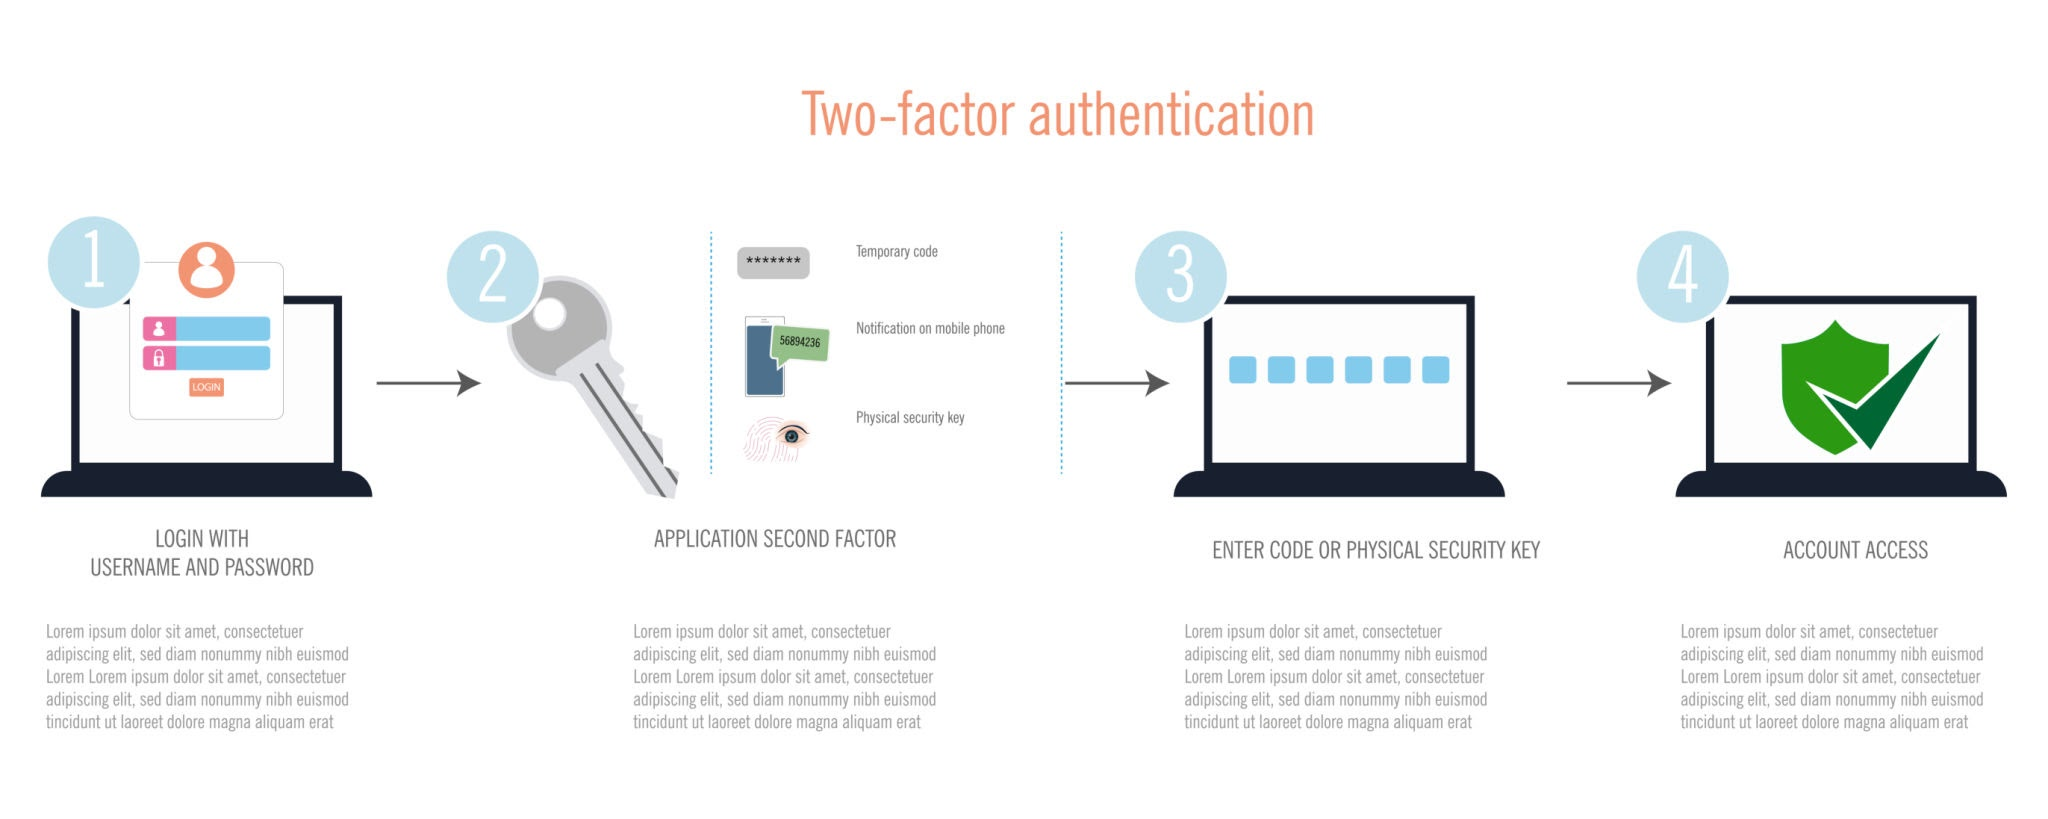
\includegraphics[width=0.8\textwidth]{images/mfa_report.png}
    \caption{Security reports indicate that implementing MFA can prevent more than 99\% of automated account takeover attacks \cite{ref3}.}
\end{figure}

\begin{itemize}
    \item \textbf{Passwordless Authentication (Passwordless \& Passkeys):} This is the most advanced defense technology trend today, based on WebAuthn and FIDO standards. Instead of sharing passwords (shared secrets), Passkeys use cryptographic key pairs stored directly on the device. This method not only optimizes user experience but also completely eliminates risks such as phishing-resistant attacks and credential stuffing \cite{ref4}.
\end{itemize}

\subsubsection{Real-world Case Study: Security Transformation at Google}

To cope with the massive scale of online fraud, Google implemented a historic authentication transformation strategy:

\begin{itemize}
    \item \textbf{Phase 1:} Mandatory application of MFA for high-risk accounts (such as administrators) and expansion to general users, combined with push-based authentication to improve usability.
    
    \item \textbf{Phase 2:} Pioneered global-scale Passkey deployment. This process helped Google significantly reduce operational costs (related to password reset support and account recovery) and protect billions of users from the most sophisticated phishing techniques.
\end{itemize}

\subsection{Patch Management Process and Risk Reduction}

\subsubsection{Concept and Importance of Patch Management}

Patch Management is not simply pressing the ``update'' button on software; it is a systematic strategic process aimed at fixing security vulnerabilities before they are exploited by attackers \cite{kim2018fundamentals}.

In information security, there exists a concept called the ``Vulnerability Window'' – this is the period from when a software vulnerability is disclosed until the system is actually patched to fix that vulnerability. Delays, postponement, or ignoring the update process are the root cause that create conditions for malware to spread and cause cyberattacks on a large scale.

\subsubsection{Standard Patch Management Process}

To ensure the system is not disrupted due to compatibility issues of new updates while still closing vulnerabilities, a professional patch management process in enterprises will go through the following steps:

\begin{itemize}
    \item \textbf{Discovery \& Assessment:} Continuously monitor security bulletins to detect new vulnerabilities. Evaluate the severity of vulnerabilities for the current system.
    
    \item \textbf{Testing:} Never deploy patches directly to the entire production system. Updates must be installed in a simulated environment (Sandbox/Test environment) to ensure they do not conflict with existing business applications.
    
    \item \textbf{Deployment:} Schedule official updates, prioritizing servers/devices storing important data first.
    
    \item \textbf{Verification \& Monitoring:} Re-check to ensure the patch has been successfully applied and the system operates stably.
\end{itemize}

\subsubsection{Real-world Case Study: WannaCry Ransomware Disaster}

The WannaCry ransomware outbreak in May 2017 is the most valuable evidence of weaknesses in patch management processes of organizations worldwide \cite{ref5}.

\begin{itemize}
    \item \textbf{Vulnerability Context:} WannaCry malware was designed to automatically spread through internal networks by exploiting a critical vulnerability in the Windows SMB protocol (identifier CVE-2017-0144, also known as EternalBlue).
    
    \item \textbf{Deadly Delay:} In fact, Microsoft released a patch for this vulnerability in March 2017. However, many government agencies, hospitals, and large corporations did not perform updates in time.
    
    \item \textbf{Consequences:} More than 200,000 computers in over 150 countries were infected, all data was encrypted and ransom demanded, paralyzing healthcare and transportation systems in many countries. If the patch management process had been strictly implemented immediately when Microsoft released the update, this entire disaster could have been completely prevented from the beginning.
\end{itemize}

\subsection{Data Backup Strategy and the 3-2-1 Rule}

\subsubsection{Importance of Backup in Security}

Data backup is considered the ``last survival shield'' when outer technical defense layers fail before disasters, especially destructive attacks from ransomware. Considering under the core security model CIA Triad (CIA Triad), backup strategy plays a decisive role in protecting Availability, ensuring systems and business services can operate again in the shortest time after incidents.

\subsubsection{Gold Standard: The 3-2-1 Backup Rule}

To ensure the highest resilience against data loss risks, organizations are recommended to strictly follow the 3-2-1 rule:

\begin{itemize}
    \item \textbf{3 copies of data:} Always maintain at least three copies of important data (including 1 original copy in operation and 2 independent backup copies). Having multiple copies helps minimize the risk of total loss if one copy is corrupted or infected.
    
    \item \textbf{2 different storage media types:} Store backup copies on at least two different physical technologies or storage systems (for example: NAS and tape). This helps avoid mass hardware failure risks.
    
    \item \textbf{1 offsite backup:} It is mandatory to have at least one backup located outside the main data center (for example: Cloud or another geographic location). This is the most important protection layer against physical disasters or large-scale malware spread.
\end{itemize}

\subsubsection{Enhanced Defense: Immutable and Air-gapped Backup}

In the context of increasingly sophisticated ransomware, they not only encrypt original data but also attempt to delete backup copies connected to the system. Therefore, backup strategies must be upgraded with the following technologies:

\begin{itemize}
    \item \textbf{Immutable Backup:} Data is stored using the WORM (Write Once, Read Many) mechanism, cannot be modified or deleted within a defined period, even by administrators.
    
    \item \textbf{Air-gap:} Backup copies are completely isolated from internal networks and the Internet, only temporarily connected during backup execution.
\end{itemize}

\subsubsection{Core Benefits and Practical Application}

Implementing a proper backup strategy brings essential benefits:

\begin{itemize}
    \item Fast and accurate data recovery.
    \item Neutralizing pressure from ransomware attacks.
    \item Ensuring business continuity.
\end{itemize}

\textbf{Real-world example:} An enterprise is attacked by ransomware causing all data to be encrypted. Thanks to applying the 3-2-1 rule with backup copies on Cloud, the IT team isolated the system, restored data from a clean backup copy and brought the system back to operation within only a few hours without paying ransom.

\subsection{Incident Response Lifecycle}

\subsubsection{Importance of Incident Response}

No matter how well an organization deploys Defense-in-Depth architecture, the risk of intrusion always exists. When an incident occurs (for example: a server is infected with malware, an administrator account is stolen), time is the core factor. A standardized Incident Response (IR) process will help the organization move from a ``passive, panicked'' state to a ``proactive controlled'' state, with the goal: early detection of incidents, minimizing impact as much as possible, and restoring systems quickly.

\subsubsection{Six Phases of the Incident Response Lifecycle}

A complete incident response lifecycle includes six phases:

\begin{itemize}
    \item \textbf{Preparation:} Establish a CSIRT team, build response playbooks, deploy monitoring tools and ensure backup systems are operational.
    
    \item \textbf{Detection:} Use SIEM or log systems to detect abnormal signs (for example: multiple failed login attempts or sudden increase in encrypted traffic).
    
    \item \textbf{Containment:} Isolate infected devices, segment the network and lock suspicious accounts to prevent malware from spreading.
    
    \item \textbf{Eradication:} Remove malware, delete backdoors and patch exploited vulnerabilities.
    
    \item \textbf{Recovery:} Restore systems from clean backup copies and monitor to ensure no reinfection occurs.
    
    \item \textbf{Lesson Learned:} Analyze root causes and upgrade the system (for example: transition from SFA to MFA).
\end{itemize}

\subsubsection{Real-world Example (Ransomware Response Scenario)}

An employee is tricked into downloading malware from a phishing email:

\begin{itemize}
    \item The EDR system detects abnormal encryption processes (Detection).
    \item The computer is isolated from the internal network (Containment).
    \item The IT team removes malware and cleans the system (Eradication).
    \item Data is restored from Cloud backup (Recovery).
    \item The company organizes anti-phishing training and upgrades authentication (Lesson Learned).
\end{itemize}

\subsection{User Awareness and Security Recommendations}

\subsubsection{Humans: The Weakest Link}

In any information system, no matter how perfectly Defense-in-Depth architecture is designed, humans are always considered the ``weakest link'' in the security chain. Instead of directly attacking technical systems, attackers often use Social Engineering techniques to manipulate users \cite{ref1}.

\subsubsection{Common Risky Behaviors}

Common mistakes that users often make include:

\begin{itemize}
    \item \textbf{Phishing:} Clicking on fraudulent links leading to credential theft or malware installation.
    
    \item \textbf{Downloading Malicious Software:} Installing cracked software or from untrusted sources.
    
    \item \textbf{Weak Passwords:} Using easily guessable passwords or reusing passwords.
    
    \item \textbf{Ignoring Updates:} Not updating systems, creating vulnerabilities for hackers to exploit.
\end{itemize}

\subsubsection{Recommendations and Solutions}

\textbf{For End Users:}
\begin{itemize}
    \item Use strong passwords and enable MFA.
    \item Participate in periodic security awareness training.
\end{itemize}

\textbf{For Technical Departments:}
\begin{itemize}
    \item Deploy SIEM, EDR for monitoring.
    \item Apply Network Segmentation.
\end{itemize}

\subsection{Future Trends and Conclusion}

\subsubsection{Emerging Cybersecurity Threats}

Modern attack trends include:

\begin{itemize}
    \item \textbf{AI-powered Malware:} Using AI to create sophisticated malware and phishing.
    
    \item \textbf{Fileless \& Living-off-the-Land:} Attacks without files, using system tools such as PowerShell.
    
    \item \textbf{Ransomware 3.0 \& Supply Chain Attack:} Attacks through supply chains (example SolarWinds).
\end{itemize}

\subsubsection{Overall Conclusion}

Cybersecurity threats are increasingly sophisticated and dangerous. Protecting systems cannot rely on a single solution.

To ensure the three core elements of information security:

\begin{itemize}
    \item Confidentiality
    \item Integrity
    \item Availability
\end{itemize}

Organizations need to:

\begin{itemize}
    \item Deploy multi-layered defense (Defense-in-Depth)
    \item Upgrade authentication (MFA, Passkey)
    \item Build operational and incident response processes
    \item Enhance user awareness
\end{itemize}




\newpage
\section{Future Trends in Malicious Software}

\newpage
\section{Conclusion}

The study of Chapter 8 shows that malicious software has changed from a small technical problem into a professional criminal tool. As malware becomes smarter, our ways of defending must also improve.

\subsection{Final Summary of Key Lessons}

Through our research, we can conclude three main things:

\begin{itemize}
  \item Technology is not the only answer: We can have the best firewalls, but Social Engineering (tricking people) is still the easiest way for hackers to get in. Educating users (User Awareness) is the most important layer of defense [1].
  \item Protecting the CIA Triad: Every attack we studied targets the pillars of security. Spyware breaks Confidentiality, Viruses break Integrity, and Ransomware destroys Availability. A good security plan must protect all three [1].
  \item Focus on Resilience: Since threats like "Fileless" and "AI malware" are hard to stop, organizations must focus on Cyber Resilience. This means being ready to recover quickly using a strong 3-2-1 Backup Strategy and a clear Incident Response plan.
\end{itemize}

\subsection{The Reality in Vietnam}

The 2024-2025 Ransomware attacks in Vietnam, which hit companies like VNDIRECT and PVOIL, prove that the theories in Chapter 8 are very real. These attacks caused huge losses and showed that Vietnamese businesses must implement Defense in Depth immediately to survive in the digital age.

\subsection{Final Words}

Malware will never stop evolving. However, by staying proactive with Patch Management, using modern AI-based defense tools, and constantly teaching users to be careful, we can stay safe. Security is not a one-time job; it is a continuous journey of learning and adapting.


\FloatBarrier

\newpage

% \begin{thebibliography}{99}

% \bibitem{nist} National Institute of Standards and Technology. (2017). \textit{Digital Identity Guidelines: Authentication and Lifecycle Management}. NIST SP 800-63-3.

% \bibitem{owasp} OWASP Foundation. (2021). \textit{OWASP Top 10 Web Application Security Risks}. Retrieved from https://owasp.org/www-project-top-ten/

% \bibitem{schneier} Schneier, B. (2015). \textit{Data and Goliath: The Hidden Battles to Collect Your Data and Control Your World}. W. W. Norton \& Company.

% \bibitem{stallings} Stallings, W. (2016). \textit{Cryptography and Network Security: Principles and Practice} (7th ed.). Pearson.

% \bibitem{ferguson} Ferguson, N., Schneier, B., \& Kohno, T. (2010). \textit{Cryptography Engineering: Design Principles and Practical Applications}. Wiley Publishing.

% \bibitem{iso27001} International Organization for Standardization. (2013). \textit{Information technology – Security techniques – Information security management systems – Requirements}. ISO/IEC 27001:2013.

% \bibitem{iso27035} International Organization for Standardization. (2016). \textit{Information technology – Security techniques – Information security incident management}. ISO/IEC 27035:2016.

% \bibitem{cisa} Cybersecurity and Infrastructure Security Agency. (2021). \textit{Authentication Best Practices}. Retrieved from https://www.cisa.gov/

% \bibitem{sans} SANS Institute. (2020). \textit{Authentication and Authorization for Cloud-Based Applications}. SANS Security Essentials.

% \bibitem{zerotrast} Rose, S., Borchert, O., Mitchell, S., \& Connelly, S. (2020). \textit{Zero Trust Architecture}. NIST SP 800-207.

% \end{thebibliography}

% === file này không sửa gì vào nha, thêm ref ở file ref.bib

\cleardoublepage
\phantomsection
\addcontentsline{toc}{section}{References}
\nocite{*}
\bibliographystyle{unsrt}
\bibliography{ref}



\end{document}


